\documentclass[10pt]{ctexart}
\usepackage{NotesTeX}

%\usepackage{showframe}

\title{\begin{center}{\Huge \textit{电力系统分析}}\\{{\itshape Power System}}\end{center}}
\author{Seastian Ludwig\footnote{\href{https://geodesick.com/}{\textit{My Personal Website}}}}


\affiliation{
   University of Northeast Electronic Power University\\
Electronic Engineer school\\
}

\emailAdd{2019301011016@neepu.edu.cn}
\begin{document}
\maketitle
\flushbottom
\newpage
\pagestyle{fancynotes}

\part{电力系统基本概念}
\section{电力系统基本参量和接线图}
\begin{enumerate}
    \item 总装机量
    \item 年发电量
    \item 最大负荷
    \item 额定频率
    \item 电压等级
    \item 地理接线图
    \item 电气接线图
\end{enumerate}
\section{电力系统运行应满足的基本要求}
\subsection{电能的特点}
\begin{enumerate}
    \item 电能的生产输送和消耗几乎同时完成
    \item 电力系统的运行,控制,保护十分复杂
    \begin{enumerate}
        \item 数据量大
        \item 大规模数学优化问题
        \item 暂态过程短
    \end{enumerate}
    \item 运行中要保证电能的质量符合要求
    \begin{enumerate}
        \item 电压幅值
        \item 交变电压频率
        \item 电压/电流波形
    \end{enumerate}
\end{enumerate}
\section{电力系统的接线方式}
\newpage
\part{电力系统的数学模型}
\section{电力传输线物理参数模型}
\subsection{单根导线}
\begin{margintable}
    {\color{red}架空输电线路}
\end{margintable}
\begin{remark}

    \begin{enumerate}

        \item 电流热效应——电阻$ r $ 
        \item 载流导线周围磁场效应——电抗$ x $ 
        \item 线路电压施加于绝缘介质产生的泄露电流和电晕效应产生——电导$ g $ 
        \item 带电导线周围电场——电纳$ b $ 
    \end{enumerate}
\end{remark}
\begin{definition}
    单位长度导线的电阻:$$	r _{1} =\frac{\rho}{S}$$ 
    温度修正$$	r_{1} =r_{20} [1+\alpha(t-20)]$$ 
\end{definition}
\begin{margintable}
    温度影响不显著,大部分计算可以忽略温度的影响
\end{margintable}
\begin{definition}
    电抗:$$	x=2\pi f_{N} L$$ 
\end{definition}
\begin{lemma}
    经验公式:
    $$	x_{1} =0.1445 lg \frac{D_{m} }{r}+0.0157$$ 
\end{lemma}
\begin{definition}
    电导:
    $$	U_{er} =E_{er} r\ln \frac{D_{m} }{r}=49.3m_{1} m_{2} \delta r \ln \frac{D_{m} }{r}$$ 
\end{definition}
\begin{margintable}
    $ U_{er}  $临界电压 
\end{margintable}
\begin{definition}
    电纳:

    与单位导线周围的电场有关:
    $$	g_{1} =\Delta P_{g} /U^{2} \times 10^{-3} $$ 
\end{definition}
\begin{margintable}
    $ \Delta P_{g}  $ 三相电路每公里的电晕损耗
\end{margintable}
采用分裂导线降低电晕放电和线路电抗,采用分裂导线的形式(分成若干根,相互之间保持一定距离0.2~0.5m,2~4根)\\


\subsection{分裂导线}
电阻计算公式不变,由于交流电的趋肤效应,分裂导线的电阻应更小
\begin{definition}
    分裂导线的电抗:

    \begin{enumerate}
        \item 有效半径:$$	r _{eq} =\sqrt[n]{r(D_{12} D_{13} ...D_{1n} )}=\sqrt[n]{rD_{1m} ^{(n-1)} }$$ 
        \item $$ x_{1} =0.1445\lg \frac{D_{m} }{r_{eq} }+\frac{0.0157}{n} $$ 
    \end{enumerate}
\end{definition}
\begin{marginfigure}
        \centering
        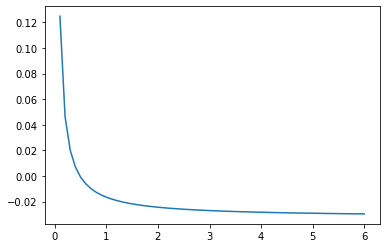
\includegraphics[scale=0.4]{figure/1x1n.png}
        \caption{$ x_{1}-n $ }
        \label{x1_n}
\end{marginfigure}
\begin{definition}
    分裂导线电纳:
    $$ b_{1} =\frac{7.58}{\lg  \frac{D_{m} }{r_{eq} }}\times 10^{-6} $$ 
\end{definition}

\section{分布参数电路等效模型}
\begin{equation}
\left\{
\begin{array}{ll}
    \frac{{\rm d}\dot{U}}{{\rm d}\dot{x}}=&z_{1} \dot{I}\\
    \frac{{\rm d}\dot{I}}{{\rm d}\dot{x}}=&y_{1} \dot{U}
\end{array}
\right.
\end{equation}
\newpage
\part{潮流计算}
\textbf{Power Flow}
\end{document}